% ==== Document Class & Packages =====
\documentclass[12pt,hidelinks]{article}
	\usepackage[explicit]{titlesec}
	\usepackage{titletoc}
	\usepackage{tocloft}
	\usepackage{charter}
	\usepackage[many]{tcolorbox}
	\usepackage{amsmath}
	\usepackage{graphicx}
	\usepackage{xcolor}
	\usepackage{tikz,lipsum,lmodern}
	\usetikzlibrary{calc}
	\usepackage[portuguese]{babel}
	\usepackage{fancyhdr}
	\usepackage{mathrsfs}
	\usepackage{empheq}
	\usepackage{fourier}% change to lmodern if fourier is no available
	\usepackage{wrapfig}
	\usepackage{fancyref}
	\usepackage{hyperref}
	\usepackage{cleveref}
	\usepackage{listings}
	\usepackage{varwidth}
	\usepackage{longfbox}
	\usepackage{geometry}
	\usepackage{marginnote}
	\usepackage{float}
	\usepackage[utf8]{inputenc}
	\usepackage[T1]{fontenc}
	\usepackage[alf]{abntex2cite}
	\usepackage{caption}
	
	\tcbuselibrary{theorems}
	\tcbuselibrary{breakable, skins}
	\tcbuselibrary{listings, documentation}
	\geometry{
		a4paper,
		left=33mm,
		right=33mm,
		top=20mm}

% Custom captions


% ========= Path to images ============
%   - Direct the computer on the path 
% 	  to the folder containg the images
% =====================================
\graphicspath{{./imagens/}}
% ============= Macros ================
\newcommand{\fillin}{\underline{\hspace{.75in}}{\;}}
\newcommand{\solution}{\textcolor{mordantred19}{Solution:}}
\setlength{\parindent}{0pt}
\addto{\captionsenglish}{\renewcommand*{\contentsname}{Sumário}}
\addto{\captionsportuguese}{\renewcommand*{\contentsname}{Sumário}}
\addto\captionsportuguese{\renewcommand{\bibname}{Bibliografia}}
\addto\captionsportuguese{\renewcommand{\refname}{Bibliografia}}
\linespread{1.2}
% ======== Footers & Headers ==========
\cfoot{\thepage}
\chead{}\rhead{}\lhead{}
% =====================================
\renewcommand{\thesection}{\arabic{section}}
\newcommand\sectionnumfont{% font specification for the number
	\fontsize{380}{130}\color{myblueii}\selectfont}
\newcommand\sectionnamefont{% font specification for the name "PART"
	\normalfont\color{white}\scshape\small\bfseries }
% ============= Colors ================
% ----- Red -----
\definecolor{mordantred19}{rgb}{0.68, 0.05, 0.0}
% ----- Blue -----
\definecolor{st.patrick\'sblue}{rgb}{0.14, 0.16, 0.48}
\definecolor{teal}{rgb}{0.0, 0.5, 0.5}
\definecolor{beaublue}{rgb}{0.74, 0.83, 0.9}
\definecolor{mybluei}{RGB}{0,173,239}
\definecolor{myblueii}{RGB}{63,200,244}
\definecolor{myblueiii}{RGB}{199,234,253}
% ---- Yellow ----
\definecolor{blond}{rgb}{0.98, 0.94, 0.75}
\definecolor{cream}{rgb}{1.0, 0.99, 0.82}
% ----- Green ------
\definecolor{emerald}{rgb}{0.31, 0.78, 0.47}
\definecolor{darkspringgreen}{rgb}{0.09, 0.45, 0.27}
% ---- White -----
\definecolor{ghostwhite}{rgb}{0.97, 0.97, 1.0}
\definecolor{splashedwhite}{rgb}{1.0, 0.99, 1.0}
% ---- Grey -----
\definecolor{whitesmoke}{rgb}{0.96, 0.96, 0.96}
\definecolor{lightgray}{rgb}{0.92, 0.92, 0.92}
\definecolor{floralwhite}{rgb}{1.0, 0.98, 0.94}
% ========= Part Format ==========
\titleformat{\section}
{\normalfont\huge\filleft}
{}
{20pt}
{\begin{tikzpicture}[remember picture,overlay]
	\fill[myblueiii] 
	(current page.north west) rectangle ([yshift=-13cm]current page.north east);   
\node[
	fill=mybluei,
	text width=2\paperwidth,
	rounded corners=6cm,
	text depth=18cm,
	anchor=center,
	inner sep=0pt] at (current page.north east) (parttop)
	{\thepart};%
\node[
	anchor=south east,
	inner sep=0pt,
	outer sep=0pt] (partnum) at ([xshift=-20pt]parttop.south) 
	{\sectionnumfont\thesection};
\node[
	anchor=south,
	inner sep=0pt] (partname) at ([yshift=2pt]partnum.south)   
	{\sectionnamefont CAPÍTULO};
\node[
	anchor=north east,
	align=right,
	inner xsep=0pt] at ([yshift=-0.5cm]partname.east|-partnum.south) 
	{\parbox{.7\textwidth}{\raggedleft#1}};
\end{tikzpicture}%
}
% ========= Hyper Ref ===========
\hypersetup{
	colorlinks,
	linkcolor={red!50!black},
	citecolor={blue!50!black},
	urlcolor={blue!80!black}
}
% ========= Example Boxes =============
\tcbset{
	defstyle/.style={
		fonttitle=\bfseries\upshape, 
		fontupper=\slshape,
		arc=0mm, 
		beamer,
		colback=blue!5!white,
		colframe=blue!75!black},
	theostyle/.style={
		fonttitle=\bfseries\upshape, 
		fontupper=\slshape,
		colback=red!10!white,
		colframe=red!75!black},
	visualstyle/.style={
		height=6.5cm,
		breakable,
		enhanced,
		leftrule=0pt,
		rightrule=0pt,
		bottomrule=0pt,
		outer arc=0pt,
		arc=0pt,
		colframe=mordantred19,
		colback=lightgray,
		attach boxed title to top left,
		boxed title style={
			colback=mordantred19,
			outer arc=0pt,
			arc=0pt,
			top=3pt,
			bottom=3pt,
		},
		fonttitle=\sffamily,},
	discussionstyle/.style={
		height=6.5cm,
		breakable,
		enhanced,
		rightrule=0pt,
		toprule=0pt,
		outer arc=0pt,
		arc=0pt,
		colframe=mordantred19,
		colback=lightgray,
		attach boxed title to top left,
		boxed title style={
			colback=mordantred19,
			outer arc=0pt,
			arc=0pt,
			top=3pt,
			bottom=3pt,
		},
		fonttitle=\sffamily},
	mystyle/.style={
		height=6.5cm,
		breakable,
		enhanced,
		rightrule=0pt,
		leftrule=0pt,
		bottomrule=0pt,
		outer arc=0pt,
		arc=0pt,
		colframe=mordantred19,
		colback=lightgray,
		attach boxed title to top left,
		boxed title style={
			colback=mordantred19,
			outer arc=0pt,
			arc=0pt,
			top=3pt,
			bottom=3pt,
		},
		fonttitle=\sffamily},
	aastyle/.style={
			height=3.5cm,
			enhanced,
			colframe=teal,
			colback=lightgray,
			colbacktitle=floralwhite,
			fonttitle=\bfseries,
			coltitle=black,
		attach boxed title to top center={
	  		yshift=-0.25mm-\tcboxedtitleheight/2,
	   		yshifttext=2mm-\tcboxedtitleheight/2}, 
		boxed title style={boxrule=0.5mm,
			frame code={ \path[tcb fill frame] ([xshift=-4mm]frame.west)
				-- (frame.north west) -- (frame.north east) -- ([xshift=4mm]frame.east)
				-- (frame.south east) -- (frame.south west) -- cycle; },
			interior code={ 
				\path[tcb fill interior] ([xshift=-2mm]interior.west)
				-- (interior.north west) -- (interior.north east)
				-- ([xshift=2mm]interior.east) -- (interior.south east) -- (interior.south west)
				-- cycle;} }
				},
	examstyle/.style={
		height=9.5cm,
		breakable,
		enhanced,
		rightrule=0pt,
		leftrule=0pt,
		bottomrule=0pt,
		outer arc=0pt,
		arc=0pt,
		colframe=mordantred19,
		colback=lightgray,
		attach boxed title to top left,
		boxed title style={
			colback=mordantred19,
			outer arc=0pt,
			arc=0pt,
			top=3pt,
			bottom=3pt,
		},
		fonttitle=\sffamily},
	doc head command={
		interior style={
			fill,
			left color=yellow!20!white, 
			right color=white}},
	doc head environment={
		boxsep=4pt,
		arc=2pt,
		colback=yellow!30!white,
		},
	doclang/environment content=text
}
% ============= Boxes ================
\newtcolorbox[auto counter,number within=section]{example}[1][]{
	mystyle,
	title=Prática~\thetcbcounter,
	overlay unbroken and first={
		\path
		let
		\p1=(title.north east),
		\p2=(frame.north east)
		in
		node[anchor=
			west,
			font=\sffamily,
			color=st.patrick\'sblue,
			text width=\x2-\x1] 
		at (title.east) {#1};
	}
}
\newtcolorbox[auto counter,number within=section]{longexample}[1][]{
	examstyle,
	title=Example~\thetcbcounter,
	overlay unbroken and first={
		\path
		let
		\p1=(title.north east),
		\p2=(frame.north east)
		in
		node[anchor=
		west,
		font=\sffamily,
		color=st.patrick\'sblue,
		text width=\x2-\x1] 
		at (title.east) {#1};
	}
}
\newtcolorbox[auto counter,number within=section]{example2}[1][]{
	aastyle,
	title=Example~\thetcbcounter,{}
}
\newtcolorbox[auto counter,number within=section]{discussion}[1][]{
	discussionstyle,
	title=Discussion~\thetcbcounter,
	overlay unbroken and first={
		\path
		let
		\p1=(title.north east),
		\p2=(frame.north east)
		in
		node[anchor=
		west,
		font=\sffamily,
		color=st.patrick\'sblue,
		text width=\x2-\x1] 
		at (title.east) {#1};
	}
}
\newtcolorbox[auto counter,number within=section]{visualization}[1][]{
	visualstyle,
	title=Visualization~\thetcbcounter,
	overlay unbroken and first={
		\path
		let
		\p1=(title.north east),
		\p2=(frame.north east)
		in
		node[anchor=
		west,
		font=\sffamily,
		color=st.patrick\'sblue,
		text width=\x2-\x1] 
		at (title.east) {#1};
	}
}
% --------- Theorems ---------
\newtcbtheorem[number within=subsection,crefname={definition}{definitions}]%
	{Definition}{Definition}{defstyle}{def}%
\newtcbtheorem[use counter from=Definition,crefname={theorem}{theorems}]%
	{Theorem}{Theorem}{theostyle}{theo}
	%
\newtcbtheorem[use counter from=Definition]{theo}{Theorem}%
{
	theorem style=plain,
	enhanced,
	colframe=blue!50!black,
	colback=yellow!20!white,
	coltitle=red!50!black,
	fonttitle=\upshape\bfseries,
	fontupper=\itshape,
	drop fuzzy shadow=blue!50!black!50!white,
	boxrule=0.4pt}{theo}
\newtcbtheorem[use counter from=Definition]{DashedDefinition}{Definition}%
 {
 	enhanced,
 	frame empty,
 	interior empty,
 	colframe=darkspringgreen!50!white,
	coltitle=darkspringgreen!50!black,
	fonttitle=\bfseries,
	colbacktitle=darkspringgreen!15!white,
	borderline={0.5mm}{0mm}{darkspringgreen!15!white},
	borderline={0.5mm}{0mm}{darkspringgreen!50!white,dashed},
	attach boxed title to top center={yshift=-2mm},
	boxed title style={boxrule=0.4pt},
	varwidth boxed title}{theo}
%%%%%%%%%%%%%%%%%%%%%%%%%%%%%%%%%%%%%%%%
\newtcblisting[auto counter,number within=section]{disexam}{
	skin=bicolor,
	colback=white!30!beaublue,
	colbacklower=white,
	colframe=black,
	before skip=\medskipamount,
	after skip=\medskipamount,
	fontlower=\footnotesize,
	listing options={style=tcblatex,texcsstyle=*\color{red!70!black}},}
%%%%%%%%%%%%%%%%%%%%%%%%%%%%%%%%%%%%%%%

\begin{document}
\begin{titlepage}
	\centering % Center everything on the title page
	\scshape % Use small caps for all text on the title page
	\vspace*{1.5\baselineskip} % White space at the top of the page

	{\large Instituto Federal de Educação, Ciência e Tecnologia de Minas Gerais }
	
% ===================
%	Title Section 	
% ===================

	\rule{13cm}{1.6pt}\vspace*{-\baselineskip}\vspace*{2pt} % Thick horizontal rule
	\rule{13cm}{0.4pt} % Thin horizontal rule
	
		\vspace{0.75\baselineskip} % Whitespace above the title
% ========== Title ===============	

	{	\Huge Introdução a Forense Digital\\
	          e Resposta a Incidentes\\	}
% ======================================
		\vspace{0.75\baselineskip} % Whitespace below the title
	\rule{13cm}{0.4pt}\vspace*{-\baselineskip}\vspace{3.2pt} % Thin horizontal rule
	\rule{13cm}{1.6pt} % Thick horizontal rule
	
		\vspace{1.75\baselineskip} % Whitespace after the title block

% ========= Autores ==============

	{\large Mário Luiz Rodrigues Oliveira e \\
	Rafael Alvarenga de Azevedo} \\

\end{titlepage}
%%%%%%%%%%%%%%%%%%%%%%%%%%%%%%%%%%%%%%%%%%%%%%%%%%%%%%%%%%%
\tableofcontents
\vfill

\newpage
\newgeometry{
	left=29mm, 
	right=29mm, 
	top=20mm, 
	bottom=15mm}


%%%%%%%%%%%%%%%%%%%%%%%%%%%%%%%%%%%%%%%%%%%%%%%%%%%%%%%%%%%
\section{Introdução}

    \vspace{10.5cm}

    \hspace{1cm}
    Com o advento da rede mundial de computadores, a sociedade contemporânea passou a ter facilidade no acesso a diversas fontes de informação. Sem dúvida, tal inovação contribuiu no processo de globalização das economias do século XXI. No entanto, não somente a população comum passou a produzir e consumir informações, como também agentes maliciosos tentam, frequentemente, ter acesso não autorizado a tais dados. Sendo assim, um país em busca de garantir a segurança das informações de sua população, deve adequar os crimes cibernéticos em sua constituição. Além disso, deve treinar novos especialistas para lidar com essa categoria de delito.
        
    \vspace{4mm}
    
    \hspace{1cm}
    A Forense Digital é o campo do conhecimento em que se estuda procedimentos científicos para auxiliar na investigação de crimes cometidos com o emprego de dispositivos digitais. O perito é responsável por coletar, examinar, analisar e relatar possíveis evidências encontradas em um eletrônico.
    
    \vspace{4mm}
	
	\hspace{1cm}
	Resposta a Incidentes é o ramo da Segurança da Informação especializado na procura por maneiras de mitigar ataques advindos de atores maliciosos na \textit{Internet}. Além disso, pode usar técnicas e ferramentas forenses para formalizar seu processo de investigação. Portanto, quando se fala em Forense Digital e Resposta a Incidentes (FDRI), entende-se a utilização de aparatos teórico-práticos de Forense Digital na resolução de problemas decorrentes de incidentes cibernéticos.
    
    \vspace{4mm}
	
	\hspace{1cm}
	Por meio do entendimento do processo forense clássico, percebe-se que é possível aplicá-lo na tentativa de gerar uma resposta a um ataque ocorrido. Por conseguinte, para melhor compreensão do assunto, propõe-se o estudo das seguintes subáreas de FDRI: análise de sistema de arquivos; análise de memória volátil; análise de redes de computadores; análise de logs; análise de inteligência e análise de malware.
    
    \vspace{4mm}
    
    \hspace{1cm}
    Na análise forense de sistemas de arquivos é possível entender o que estava sendo usado em um computador. Ter conhecimento de como verificar o que está contido em memória volátil é crucial para tratar casos em que criminosos utilizam este tipo de tecnologia para operar. Forense em redes de computadores é essencial para extrair informações de diferentes hospedeiros envolvidos com um incidente. A análise de logs de um sistema é pertinente para identificar eventos no mesmo. O exame de todo tipo de informação sobre um atacante é relevante para tratar com dada ameaça cibernética. Análise de malware é útil para extrair informações de programas maliciosos.
    
    \vspace{4mm}
	
	\hspace{1cm}
	Do capítulo 2 ao capítulo 7 há uma introdução a cada uma das subáreas dispostas. Ao final de cada um, há exercícios para que o leitor possa reforçar o conteúdo estudado. Dessa forma, espera-se que o aluno seja introduzido na área de FDRI. Entretanto, recomendamos que o estudante faça uma revisão de alguns conceitos de computação, através dos tópicos contidos na subseção \ref{cap1_visao_geral}.
	
   \subsection{Forense Digital}
    
    \hspace{1cm}
    Como define \citeonline{vecchia2019}, a forense digital, ou perícia forense, possui um conjunto de técnicas e procedimentos com embasamento científico para coletar, analisar e expor os indícios encontrados no processo de reconstrução de ações executadas em dispositivos digitais. Adotaremos o processo forense proposto pelo NIST, explicitado na subseção \ref{cap1_visao_geral_procfor}. Outrossim, existem tipos distintos de profissionais nesta área, e todos utilizam um método bem elaborado para efetuar uma perícia. Esta, pode ser feita em equipamentos desligados, ligados ou conectados a Internet, com as devidas ferramentas.
    
    \vspace{4mm}
        
    \hspace{1cm}
    O estudante de tecnologia da informação, que foca nessa área, pode atuar no mercado através de uma das quatro denominações de perito: oficial (passa por concurso público), \textit{ad hoc} (nomeado por um juiz), assistente técnico (contratado pelas partes envolvidas em um processo) ou privado (contratado por uma pessoa, antes de levar o caso para o judiciário). De modo a normalizar as técnicas utilizadas por esses profissionais, é adotado, internacionalmente, uma estratégia com enfoque na garantia de integridade das mídias digitais coletadas \cite{vecchia2019}.
    
    \subsection{Resposta a Incidentes} \label{cap1_ir}
    
    \hspace{1cm}
    A área de Resposta a Incidentes é aquela que realiza uma abordagem coordenada e estruturada que compreende desde a detecção de um incidente até sua resolução (resposta) \cite{luttgens2014}. Ainda, é uma profissão multidisciplinar que foca em identificar, investigar, e remediar a exploração de redes de computadores \cite{roberts2016}.

    \vspace{4mm}

    \hspace{1cm}
    Como proposto por \citeonline{luttgens2014}, para responder a um incidente, emprega-se um processo que compreende 3 etapas principais: resposta inicial, investigação e remediação. Na primeira etapa, busca-se agregar o maior número de informações sobre um incidente ocorrido. Para isso, utilizam-se informações da rede no momento do ataque, como \textit{logs} de rede \cite{luttgens2014}. Tendo identificado o incidente, as duas fases subsequentes ocorrem de forma concorrente, em busca de responder ao acometimento dos sistemas.
        
    \vspace{4mm}
    
    \hspace{1cm}
    Além das 3 etapas principais, \citeonline{luttgens2014} projetaram um processo iterativo para manutenção da fase de investigação, como mostra a figura \ref{IR_lifecycle}. Para fins didáticos, vamos nos concentrar nas subetapas de Coleta de Evidências e Análise de Dados. A coleta de evidências ocorre em função de um processo padronizado que preserva a integridade das informações. Ademais, uma organização pode modificar tal processo para atender demandas internas \cite{luttgens2014}. Como posto anteriormente, escolhemos o processo clássico do NIST para estudarmos. Finalmente, na fase de análise dos dados, busca-se extrair informações relevantes para tentar mitigar o incidente ocorrido, ao responder perguntas feitas na investigação.
    
    \begin{figure}[H]
    	\centering
    	\caption{Ciclo de vida da investigação de um incidente}
    	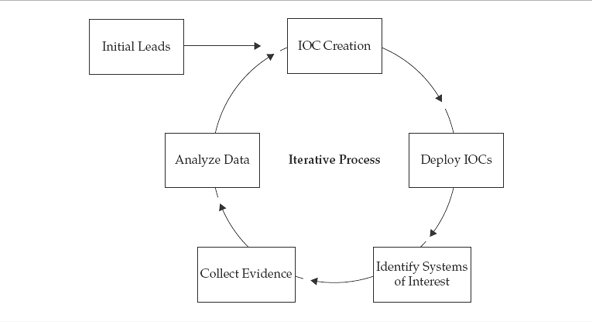
\includegraphics[scale=1]{IR_investigation}
    	\caption*{Fonte: \citeonline{luttgens2014}}
    	\label{IR_lifecycle}
    \end{figure}
    
    \subsection{Visão Geral} \label{cap1_visao_geral}
    
    \hspace{1cm}
    Antes de começar a leitura dos capítulos específicos, recomendamos que você faça uma revisão dos conceitos envolvidos com cada subárea de FDRI. Primeiramente, apresentaremos o Processo Forense Clássico proposto pelo NIST. Em seguida, explicaremos o que é Sistema de Arquivo e para que serve; o que é a Memória Principal de um computador; como são formadas as Redes de Computadores; e o que são códigos maliciosos.
    
    \subsubsection{Processo Forense Clássico} \label{cap1_visao_geral_procfor}
    
    \hspace{1cm}
    Para ser possível reconstruir as ações de um usuário em determinado dispositivo, adota-se um \textit{Processe Forense} padronizado por uma entidade de renome, para garantir que as evidências coletadas configurem um relatório pericial. Este, é então levado para uma parte interessada, que dará continuidade na investigação corrente.

    \vspace{4mm}

    \hspace{1cm}
    O \textit{Processo Forense}, internacionalmente utilizado, é aquele proposto pela entidade norte-americana NIST. Ele é constituído das seguintes etapas: Coleta, Exame, Análise e Relatório (como ilustra a imagem \ref{nist_proc}).

    \begin{figure}[H]
    	\centering
    	\caption{Processo forense clássico}
    	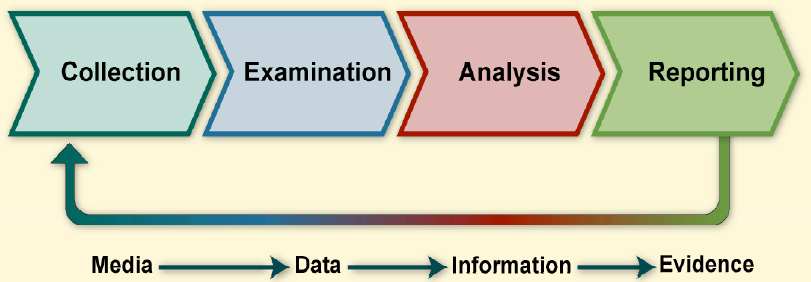
\includegraphics[scale=0.7]{nist_process}
    	\caption*{Fonte: \citeonline{kent2006}}
    	\label{nist_proc}
    \end{figure}
    
    \hspace{1cm}
    Na etapa de coleta, o profissional fará a duplicação de discos rígidos ou de memórias voláteis. Por conseguinte, inicializa-se a fase de Exame dos dados duplicados, buscando-se filtrar a grande massa de dados obtida, anteriormente, de modo a coletar informações realmente relevantes para a perícia. No estágio de análise, o perito tem que examinar, de forma manual, os resultados adquiridos na fase anterior. Essa análise é muito difícil de ser automatizada, pois, os dados devem constituir evidências para o relatório pericial. Por fim, com os resultados em mãos, o perito deve relatar tudo que foi obtido no processo \cite{kent2006}.
        
    \subsubsection{Sistema de Arquivos} \label{cap1_visao_geral_sa}
    
    \hspace{1cm}
    Todo computador pessoal é composto por um Sistema Operacional (SO) e um Sistema de Arquivos (SA). O primeiro é responsável por manter diferentes abstrações para que o usuário leigo consiga usar aplicativos em seu dia-a-dia. Já o segundo, é uma dessas abstrações, mantido  para gerir os dados do usuário, e de suas aplicações, em uma mídia de armazenamento persistente.
    
    \vspace{4mm}

    \hspace{1cm}
    Existem diversos sistemas de arquivos no mercado, cada um possui uma forma peculiar de organizar os dados do usuário em dispositivos físicos. Como o espaço destes é finito, definem-se tamanhos para cada parte armazenada pelo sistema. A menor unidade para representar informações é chamada bloco. O espaço disponível é subdividido logicamente em cabeçalho de metadados do próprio SA, e uma área de blocos de dados. Além disso, o SA também é responsável por criar as abstrações de arquivo e diretório, para o usuário final.
    
    \vspace{4mm}
    
    \hspace{1cm}
    Arquivos podem ser texto puro, codificado em algum formato como ASCII; ou \textit{bytes} armazenados para formar um arquivo binário. Alguns sistemas operacionais implementam mecanismos de identificação de tipos de arquivos, mas geralmente o cliente reconhece um arquivo pela sua extensão ou aplicação que o criou. Enquanto isso, os diretórios, ou pastas, são estruturados por meio da abstração de árvore.
    
    \vspace{4mm}
    
    \hspace{1cm}
    Todo SA implementa operações básicas para manutenção de arquivos e diretórios. O usuário comum conhece apenas as funções exibidas na interface gráfica de um SO, como criar e apagar. Porém, mais especificamente, há uma ordem lógica para manipular arquivos. Quando um dado é criado, espaço em disco precisa ser alocado, para em seguida registrar sua localização na estrutura de diretórios \cite{silberschatz2018}. Já para apagar um arquivo, o SA precisa localizá-lo na estrutura de diretórios, e então marcar seus blocos de dados como livres. Portanto, arquivos não são completamente apagados quando o usuário o deleta pela opção correspondente.
    
    \vspace{4mm}

    \hspace{1cm}
    Destacamos que os resquícios de arquivos apagados podem ser recuperados em uma análise forense por meio da técnica denominada \textit{data carving}, ou \textit{file carving} \cite{carrier2005}. Há variações de como blocos livres são gerenciados pelos SAs existentes. Mas, usualmente, programas recuperadores de dados percorrem a área de dados de um dispositivo de armazenamento, para tentar acessar blocos livres que constituem um arquivo.
    
    \subsubsection{Memória Principal}
    
    \hspace{1cm}
    Para que as aplicações do usuário final funcionem corretamente, o computador é construído utilizando uma arquitetura do conjunto de instruções de seu processador. O modelo teórico mais conhecido é a \textit{Arquitetura de Von Neumann}. Com essa abstração, o computador possui um barramento que interliga uma Unidade de Processamento Central, um módulo de dispositivos de entrada e saída de dados (E/S) e uma Memória Principal \cite{stallings2009}. Focaremos nossa revisão conceitual nessa última por enquanto.
    
    \vspace{4mm}
    
    \hspace{1cm}
    Para executar programas, o processador realiza \textit{pipelines}, mais especificamente, para buscar instruções, decodificá-las e executá-las considerando seus operadores e operandos armazenados na memória principal \cite{stallings2009}. Além desta, um processador possui memórias embutidas chamados registradores. Levando-se em consideração a hierarquia de memória organizada por \citeonline{stallings2009}, percebe-se que os registradores são mais rápidos de serem acessados pela CPU do que a memória principal. Isso se deve ao fato dessa memória transitória estar mais próxima do processador, fisicamente. No entanto, módulos de memória principal oferecem mais capacidade de armazenamento, logo, possuem papel fundamental na manutenção do mecanismo conhecido como Memória Virtual.
        
    \vspace{4mm}

    \hspace{1cm}
    De acordo com \citeonline{silberschatz2018}, a Memória Virtual é aquela encarregada de fornecer ao programador mais espaço endereçável de memória, do que seu dispositivo físico tem. Esse mecanismo aprimora o grau de multiprogramação de um computador, à medida que aparatos como paginação sob demanda e \textit{swapping} são geridos pelo sistema hospedeiro \cite{silberschatz2018}.
    
    \subsubsection{Redes de Computadores}
    
    \hspace{1cm}
    Enquanto programas são operados por usuários em computadores ao redor do mundo, no contexto de Redes de Computadores tais dispositivos são chamados sistemas finais ou hospedeiros. A rede mundial de computadores é composta por enlaces de comunicação e comutadores de pacotes. De tal maneira que um remetente consiga enviar mensagens para um destinatário, por uma rota mantida por essas equipagens.
    
    \vspace{4mm}
    
    \hspace{1cm}
    Protocolos de comunicação são empregados para garantir o funcionamento adequado da troca de mensagens pela rede. Os mais importantes são conhecidos como TCP e IP. O protocolo TCP é responsável por definir como os pacotes devem ser transportados pela rede, e o IP por criar uma hierarquia de endereçamento lógico, e repasse, para que computadores se localizem na \textit{Internet} \cite{kurose2013}. Vale ressaltar que a localização fornecida por um endereço IP não está associado a uma localização física específica no globo, mas sim a um destinatário alcançável por um remetente.
    
    \vspace{4mm}
    
    \hspace{1cm}
    O protocolo IP tem duas versões: a versão 4 e a versão 6. A primeira, também chamada IPv4, começou a ser implantada quando a \textit{Internet} surgiu, no momento em que não se previa o crescimento exacerbado do número de dispositivos a serem endereçados. Ademais, esse protocolo não garante que apenas duas partes comunicantes leiam o conteúdo de uma mensagem, tornando-se um protocolo vulnerável a ataques \textit{Man-in-the-middle}. A segunda, denominada IPv6, fora proposta para substituir sua antecedente, fornecendo criptografia no nível dos datagramas de rede, e mais combinações de endereços lógicos \cite{kurose2013}.
    
    \vspace{4mm}
    
    \hspace{1cm}
    Processos sendo executados em um hospedeiro podem se comunicar com outros sistemas finais pela rede. Para isso, emprega-se o número IP e, opcionalmente, o número de porto, ou porta. Peguemos o exemplo da ferramenta \textit{ping}. Esta implementa o protocolo ICMP que permite a um remetente enviar uma requisição \textit{echo} para um destinatário. Neste caso, o pacote de rede não é direcionado para nenhuma porta em específico, mas chega no alvo. Por outro lado, se pegarmos a \textit{Web} como caso, adota-se um nome de domínio - posteriormente traduzido em IP pelo protocolo DNS -, e o número de porto 80, para conectar clientes com sites.
    
    \vspace{4mm}
    
    \hspace{1cm}
    A democratização do acesso à informação por meio dos dispositivos móveis corroborou para o desenvolvimento das redes de computadores. Neste contexto, usuários não precisam mais de um computador de mesa, para usufruírem dos serviços fornecidos na \textit{Web}. Para que tais aplicações funcionem, existem protocolos de segurança que protegem redes sem fio. Como é o caso dos padrões WPA e WPA2, que, embora sejam vulneráveis a ataques como \textit{Evil Twin}, permitem que \textit{smartphones} de pessoas leigas se comuniquem de forma segura com o uso de algoritmos de criptografia simétrica.
    
    \vspace{4mm}
    
    \hspace{1cm}
    Todo dispositivo possui um endereço MAC de identificação. Esse valor não pode ser alterado no dispositivo, mas pode ser substituído temporariamente, para clonar o MAC de outro dispositivo. Esta técnica é usada por especialistas em redes, quando se quer obter acesso autorizado a uma rede interna que possui filtro de endereços MAC.
    
    \vspace{4mm}
    
    \hspace{1cm}
    Redes corporativas são protegidas por sistemas \textit{Firewall}. De acordo com \citeonline{kurose2013}, eles são responsáveis por isolar a rede interna da \textit{Internet}. Para isso, eles filtram pacotes de rede que entram e saem de uma sub-rede, enquanto usuários usam aplicações.

    \subsubsection{Códigos Maliciosos} \label{cap1_visao_geral_malware}

    \hspace{1cm}
    Segundo \citeonline{sikorski2012}, qualquer programa que realize alguma ação que cause danos ao seu usuário, computador ou rede pode ser considerado um código malicioso. Exemplo disso, ataques de negação de serviço, realizado com máquinas infectadas, que visam deixar um hospedeiro alvo indisponível na \textit{Internet}, através do envio massivo de pacotes de rede. 
    
    \vspace{4mm}
    
    \hspace{1cm}
    Com o emprego de programas maliciosos, atacantes podem: extorquir vítimas com o uso de \textit{ransomwares}; espionar um alvo com \textit{spywares}; enviar anúncios como spam através de \textit{adwares}; disseminar um programa malicioso chamado \textit{worm}; colocar mais \textit{malwares} no computador da vítima com o uso de \textit{trojans}, entre outros.

    \subsection{Exercícios}
    
    \begin{example}[\quad \large Introdução] \label{cap1_exercicios}
        \begin{enumerate}
            \item Quais são as etapas do Processo Forense Clássico ?
            \item Como Forense Digital e Resposta a Incidentes se relacionam ?
            \item Descreva a organização geral de um Sistema de Arquivos.
            \item Qual a importância da Memória Virtual de um computador para o usuário final ?
            \item Quais os principais protocolos de comunicação existentes na \textit{Internet} ?
            \item Defina códigos maliciosos e cite exemplos de ataques existentes.
        \end{enumerate}
    \end{example}
    
\newpage

%%%%%%%%%%%%%%%%%%%%%%%%%%%%%%%%%%%%%%%%%%%%%%%%%%%%%%%%%%%
\section{Análise de Sistema de Arquivos}
    
    \vspace{10.5cm}
    
    \hspace{1cm}
    Neste capítulo, abordaremos algumas técnicas e ferramentas para coleta e análise de dados oriundos de máquinas investigadas. Como revisado na seção \ref{cap1_visao_geral_sa}, sistemas de arquivos são responsáveis por manter as abstrações de arquivo e diretório para o usuário final. Consequentemente, quando estamos investigando um sistema, é possível descobrir o que estava sendo usado nele, à medida que vestígios digitais são coletados e analisados.
    
    \subsection{Técnicas}
    
    \hspace{1cm}
    Antes de analisar os dados de um sistema, é preciso coletá-los. Tal operação consiste em gerar pelo menos duas cópias dos dados: a original e aquela que será usada pelo perito. Além disso, deve-se manter a integridade dos dados para eles configurarem evidências no futuro. Existem duas técnicas principais para coleta de dados: Coleta Lógica e Coleta \textit{bit-a-bit}.
    
    \subsubsection{Coleta Lógica}
    
    \hspace{1cm}
    Na coleta lógica, o profissional realiza uma cópia de arquivos e diretórios de um volume lógico, mas, essa cópia não inclui arquivos apagados e blocos de dados não utilizados \cite{kent2006}.
    
    \subsubsection{Coleta \textit{bit-a-bit}}
    
    \hspace{1cm}
    De outra forma, pode ser que o profissional necessite de uma cópia exata de todo o sistema de arquivos de um sistema-alvo. Para isso, ele dispõe da técnica de coleta \textit{bit-a-bit} para copiar os dados de um disco de armazenamento, seja para outro disco, seja para um novo arquivo \cite{kent2006}.
    
    \vspace{4mm}
    
    \hspace{1cm}
    Para garantir que os dados a serem coletados  não sejam modificados pelas ações do perito, emprega-se proteção contra escrita nas mídias encontradas. Como defende \citeonline{vecchia2019}, profissionais podem trabalhar com o \textit{Tableau} (figura \ref{tableau_img}).
    
    \begin{figure}[H]
    	\centering
    	\caption{Dispositivo de proteção contra escrita (Tableau)}
    	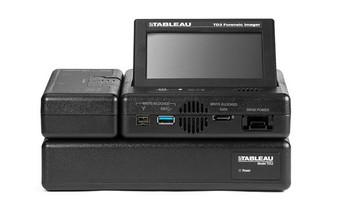
\includegraphics[scale=0.7]{img_tableau}
    	\caption*{Fonte: Google Imagens.}
    	\label{tableau_img}
    \end{figure}
    
    \subsubsection{Análise de Dados}
    
    \hspace{1cm}
    Em dada investigação sobre um incidente, uma organização pode estar interessada em revelar quais arquivos foram usados por determinado empregado, e também quando isso ocorreu. Diante disso, o analista pode classificar arquivos por nome, metadados ou conteúdo, como sugere \citeonline{carrier2005}.
    
    \vspace{4mm}
    
    \hspace{1cm}
    O nome de um arquivo sugere o que ele pode tratar. Logo, ajuda em sua classificação. Os metadados fornecem informações como tempo de acesso e permissões dadas a algum usuário. O conteúdo de um arquivo pode ser útil, quando se busca uma palavra-chave ou formato específico.
    
    \subsection{Ferramentas} \label{cap2_ferramentas}
    
    \hspace{1cm}
    Existem ferramentas como \textit{dd} e \textit{Autopsy}, que podem nos ajudar a analisar dados de um SA. Enquanto a primeira gera um arquivo de saída com a cópia de um disco, a segunda interpreta a imagem gerada e tenta classificar as informações encontradas, para facilitar sua análise.
    
    \subsubsection{Programa \textit{dd}}
    
    \hspace{1cm}
    A ferramenta \textit{dd} é disponibilizada, por padrão, nas diversas distribuições Linux. Ela é usada para fazer cópia de arquivos em um formato especificado pelo usuário. Na coleta pericial, é possível replicar discos inteiros que estejam montados no sistema hospedeiro. Dessa forma, o perito pode gerar uma cópia de um disso num formato que a ferramenta Autopsy reconheça, como o formato E01.
    
    \subsubsection{Autopsy}

    \hspace{1cm}
    Emprega-se a Autopsy para realizar o exame dos dados coletados. Esta ferramenta fornece uma interface gráfica para que o perito opere os diversos utilitários da coleção de ferramentas de linha de comando Sleuth Kit.
    
    \vspace{4mm}
    
    \hspace{1cm}
    Por meio dos \textit{Ingest Modules}, esta ferramenta disponibiliza o recurso de análise automatizada de dados, para acelerar o processo de classificação de arquivos e diretórios de uma mídia de armazenamento. Sendo assim, o operador do programa pode navegar por uma árvore de arquivos enumerados semanticamente, para examinar o conteúdo de um sistema de arquivos.

    \subsection{Exercícios}
    
    \begin{example}[\quad \large Análise de Sistema de Arquivos] \label{cap2_exercicios}
        \begin{enumerate}
            \item Quais as técnicas de coleta de dados existem para examinar dados de sistemas de arquivos ?
            \item Qual a ferramenta, dentre aquelas apresentadas na seção \ref{cap2_ferramentas}, é ideal para um perito que queira replicar os dados de um disco ?
            \item Explique o motivo pelo qual se deve manter a integridade dos dados a serem analisados em uma investigação.
            \item Para que servem os \textit{Ingest Modules} da ferramenta \textit{Autopsy} ?
        \end{enumerate}
    \end{example}
    
\newpage
%%%%%%%%%%%%%%%%%%%%%%%%%%%%%%%%%%%%%%%%%%%%%%%%%%%%%%%%%%%
\section{Análise de Memória Volátil}
    
    \vspace{10.5cm}
    
    \hspace{1cm}
    Tradicionalmente, peritos usam a técnica denominada \textit{live forensics} para coletar dados de um computador ligado na rede elétrica \cite{vecchia2019}. No entanto, no contexto corporativo de Resposta a Incidentes, técnicos podem estar interessados em saber que processos estão usando a memória principal, ou apenas duplicar os dados presentes nela naquele momento.
    
    \vspace{4mm}
    
    \hspace{1cm}
    Existem casos em que programas maliciosos dependem apenas da memória principal para funcionar, os chamados \textit{file-less malwares} \cite{wael2018}. Por conseguinte, esse aparato do sistema pode conter informações sobre programas maliciosos que estejam em operação, mas sem fornecer informações suficientes para dizer como esse programa surgiu \cite{luttgens2014}.

    \subsection{Técnicas}
    
    \hspace{1cm}
    Realizar coleta de dados da memória volátil não é uma tarefa tão simples. Deve-se ter em mente qual problema está sendo tratado e quais equipagens compõem o corpo de investigação. Em concordância com \citeonline{ligh2014}, adotaremos o diagrama apresentado pela figura \ref{diagrama_volatile} para decidir como coletar os dados desejados.
    
    \begin{figure}[H]
    	\centering
    	\caption{Diagrama de decisões para coletar dados em memória volátil}
    	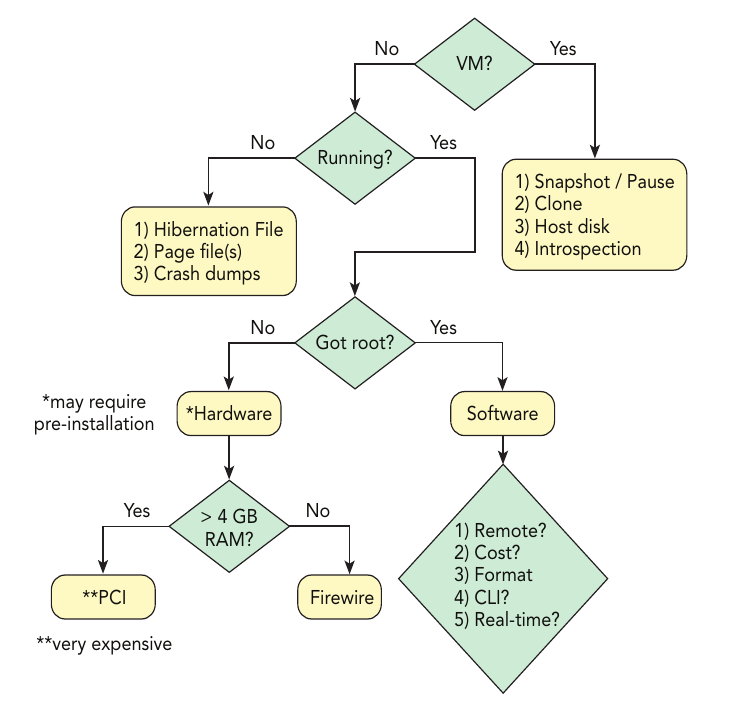
\includegraphics[scale=0.7]{img_volatile_diag}
    	\caption*{Fonte: \citeonline{ligh2014}}
    	\label{diagrama_volatile}
    \end{figure}
    
    \hspace{1cm}
    Não detalharemos todos os casos que o diagrama busca atender. Focaremos nas decisões tomadas por um perito que queira coletar a memória de um computador, sem ativar mecanismos anti-forenses adotados por \textit{rootkits} que possam estar presentes no aparelho \cite{ligh2014}.
    
    \vspace{4mm}
    
    \hspace{1cm}
    Apesar de dispositivos PCI serem caros, como defendem \citeonline{ligh2014}, eles garantem certa segurança na coleta de cópias de memória volátil, por estarem no nível lógico de dispositivos de acesso direto à memória (do inglês DMA ou \textit{Direct Memory Access}). A título de curiosidade, \citeonline{stuttgen2013} mostraram que essa forma de coleta garante que programas maliciosos não consigam adulterar o comportamento de ferramentas como a \textit{FTK Imager}. Ferramentas similares realizam um \textit{snapshot} da memória principal, e armazenam isso em alguma mídia. Dessa forma, se elas forem comprometidas, o perito não consegue prosseguir com o exame pericial.
    
    \vspace{4mm}
    
    \hspace{1cm}
    Para examinar os elementos coletados, devemos identificar qual sistema operacional estava em funcionamento. Pois, cada sistema implementa estruturas de dados diferentes para manutenção de suas aplicações. Exemplo disso, o sistema operacional Windows possui um formato de arquivos executáveis chamado PE (\textit{portable executable}). Enquanto isso, executáveis do Linux são mantidos no formato ELF.
   
    \subsection{Ferramentas}

    \hspace{1cm}
    Para examinar artefatos digitais, podemos usar a ferramenta de código aberto Volatility. Ela suporta amostras de memória volátil de sistemas operacionais como Windows, Linux, Mac OS e Android (32 bits) \cite{ligh2014}. Além disso, a ferramenta permite que pesquisadores criem \textit{plugins} que auxiliem no exame de recursos do sistema até então não suportados. Como fizeram \citeonline{case2015}, ao criarem diversos \textit{plugins} para exame especializado de diferentes estruturas internas do sistema operacional Mac OS.

    \subsection{Exercícios}
    
    \begin{example}[\quad \large Análise de Memória Volátil] \label{cap3_exercicios}
        \begin{enumerate}
            \item Explique os principais motivos pelos quais peritos podem querer coletar dados em memória volátil.
            \item A análise da memória principal de um computador pode acelerar a resolução de um incidente ? 
            \item Quais ferramentas um perito pode usar para coletar e examinar artefatos digitais ?
            \item Explique como peritos podem coletar uma amostra da memória volátil de um computador infectado por um \textit{rootkit}.
        \end{enumerate}
    \end{example}

\newpage
%%%%%%%%%%%%%%%%%%%%%%%%%%%%%%%%%%%%%%%%%%%%%%%%%%%%%%%%%%%
\section{Análise de Redes}
    
    \vspace{10.5cm}
    
    \hspace{1cm}
    A rede mundial de computadores é a ferramenta mais usada para disseminar informações. Entretanto, também possibilita diversas formas de ataques a hospedeiros vulneráveis. Entendemos por incidente um ataque ocorrido, seja ele decorrente de uma tentativa de intrusão, seja ele um evento anômalo ocorrido em uma rede interna. De qualquer forma, é necessário gerar uma resposta, para que ele não se repita e os danos causados sejam reduzidos. Para isso, precisamos analisar os vestígios digitais da rede em que sistemas finais envolvidos estão inseridos.
    
    \vspace{4mm}
    
    \hspace{1cm}
    Para analisar artefatos digitais em uma rede, precisamos relembrar dos conceitos apresentados nas seções \ref{cap1_ir} e \ref{cap1_visao_geral}. Na etapa de análise dos dados no processo de Resposta a Incidentes, é importante considerar informações de rede providas por dispositivos de acesso à \textit{Internet}, interfaces de serviços terceirizados na nuvem, sistemas de detecção de intrusão, entre outros \cite{luttgens2014}. Porém, a simples aquisição desses dados não é suficiente para auxiliar uma investigação. Consequentemente, faz-se necessária a presença do ser humano para fornecer um contexto para os dados, de uma investigação, colocados em evidência.
    
    \subsection{Técnicas}
    
    \hspace{1cm}
    A técnica denominada \textit{packet sniffing} é amplamente usada para coletar pacotes de rede. O especialista configura um receptor passivo para copiar os dados que trafegam por determinado canal de comunicação \cite{kurose2013}. Em seguida, filtra por pacotes referentes a hospedeiros e processos específicos, e os analisa.
    
    \vspace{4mm}
    
    \hspace{1cm}
    Existem bases de dados que armazenam informações aproximadas da geolocalização atual de um endereço IP da \textit{Internet}. A técnica denominada \textit{IP lookup} pode ser empregada por meio da utilização de sites que disponibilizam uma base de dados de IPs para consulta. Como exemplo, o site \href{https://www.ip-lookup.org/}{https://www.ip-lookup.org/}. 
    
    \subsection{Ferramentas} \label{cap4_ferramentas}

    \hspace{1cm}
    A ferramenta \textit{whois} fornece informações de registro de domínio de um endereço IP da \textit{Internet}. Sites como o do \href{https://registro.br/tecnologia/ferramentas/whois/}{Registro.br} podem ser usados para consultar tais informações.

    \vspace{4mm}

    \hspace{1cm}
    Organizações dispõem de \textit{Firewalls} e sistemas de detecção de intrusão (do inglês IDS ou \textit{intrusion detection system}), para tentar proteger sua rede contra ataques. Estes, 
    notificam administradores de rede sobre a quebra de alguma política de acesso \cite{bejtlich2004}.
    Aqueles, bloqueiam tentativas de conexão partidas de hospedeiros externos que estejam enviando pacotes para uma porta específica de um serviço.
    
    \vspace{4mm}
    
    \hspace{1cm}
    Porém, \textit{Firewalls} não consegue detectar anomalias originadas pela rede interna de uma empresa. Portanto, complementa-se sua utilização com os IDS. Entretanto, as ameaças mudam com o tempo, e essas ferramentas não conseguem detectar novas formas de intrusão, apenas conhecidas \cite{capobianco2019}.

    \vspace{4mm}

    \hspace{1cm}
    A filtragem pelos dados desejados pode ser feita por meio da biblioteca \textit{libpcap}. Ela é utilizada por ferramentas de captura e análise de redes, como \textit{tcpdump} e \textit{Wireshark} \cite{bejtlich2004}. Ao contrário da primeira, a segunda apresenta os pacotes trafegados na rede através de uma interface gráfica, como mostra a figura \ref{wireshark_ex}. 
    
    \begin{figure}[H]
    	\centering
    	\caption{Interface gráfica da Wireshark}
    	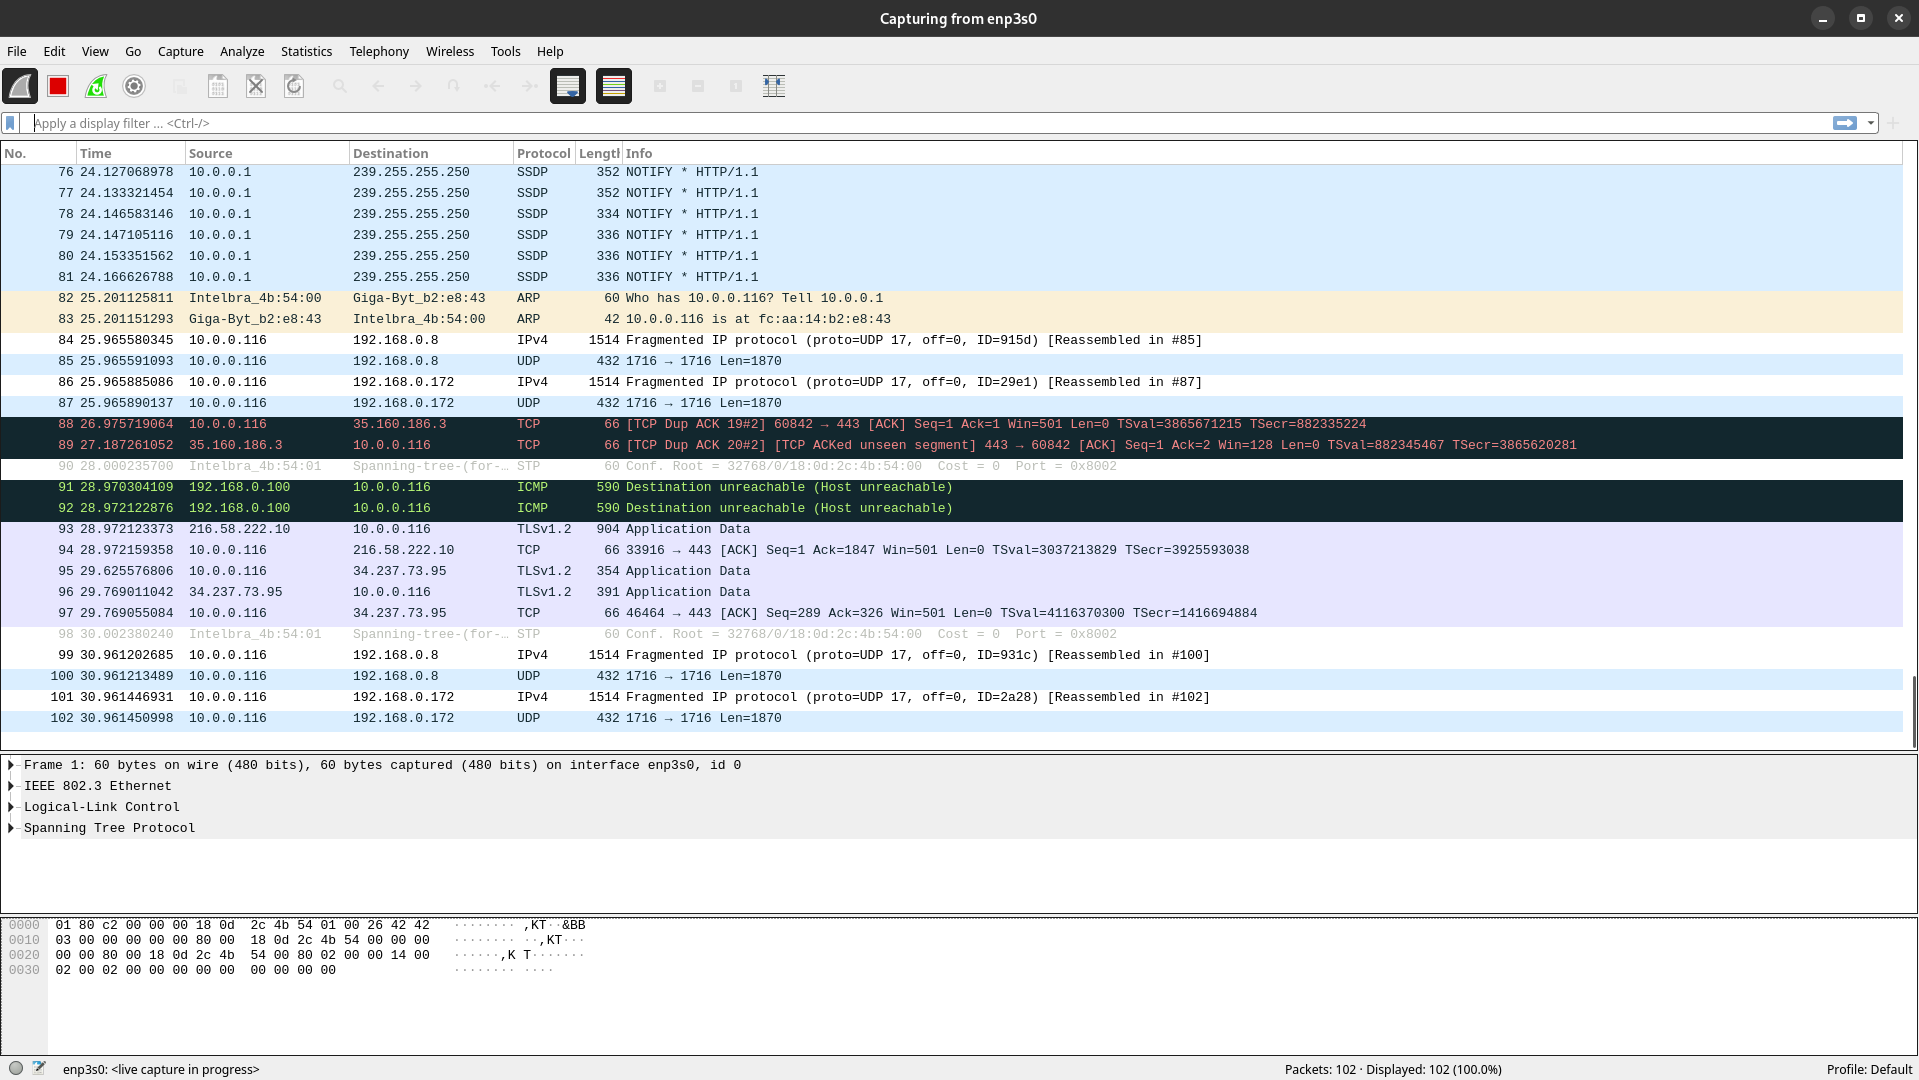
\includegraphics[scale=0.28]{img_wireshark}
    	\caption*{Fonte: próprio autor}
    	\label{wireshark_ex}
    \end{figure}

    \hspace{1cm}
    Em suma, para responder a um incidente, o profissional deve ter identificado todas as vulnerabilidades da rede, oriundas de hospedeiros comprometidos. Para tentar garantir a não reincidência de um ataque, sistemas IDS devem ser atualizados, para abranger falhas internas. Também, \textit{Firewalls} devem ser corrigidos para barrar acessos externos indesejados. Por fim, esses sistemas são mantidos por especialistas de rede, que realiza análise de pacotes e de logs de rede.

    \subsection{Exercícios}
    
    \begin{example}[\quad \large Análise de Redes] \label{cap4_exercicios}
        \begin{enumerate}
            \item O que um perito deveria fazer caso quisesse interceptar pacotes trocados por dois hospedeiros distintos na rede ?
            \item Explique a diferença entre \textit{Firewall} e sistemas de detecção de intrusão (IDS).
            \item Ao identificar o endereço IP de origem de um pacote de rede, é possível tentar localizar o hospedeiro no globo terrestre ? 
            \item Escolha um site na \textit{Internet} e consulte suas informações de domínio em \href{https://registro.br/tecnologia/ferramentas/whois/}{Registro.br}. Em seguida, 
            liste informações sobre os supostos donos de tal domínio.
        \end{enumerate}
    \end{example}

\newpage
%%%%%%%%%%%%%%%%%%%%%%%%%%%%%%%%%%%%%%%%%%%%%%%%%%%%%%%%%%%
\section{Análise de Logs}
    
    \vspace{10.5cm}
    
    \hspace{1cm}
    Aplicações distintas são projetadas para resolver determinado tipo de problema no cotidiano. Uma vez interligadas pela \textit{Internet}, informações heterogêneas são produzidas e trocadas. Para manter o devido controle do que as aplicações estão gerando em tempo de execução, desenvolvedores mantêm diferentes tipos de \textit{Logs}. Log é o nome dado para um arquivo devidamente formatado, para representar informações de: eventos ocorridos em um sistema computacional, segurança de um dispositivo, erros ocorridos na utilização de uma aplicação, instalação de programas e registros auxiliadores na depuração de \textit{softwares}.
    
    \vspace{4mm}
    
    \hspace{1cm}
    De acordo com \citeonline{kent2006}, logs podem ser classificados em cinco categorias, como seguem:
    
    \begin{itemize}
        \item \textbf{Eventos}: tipo de registro geralmente mantido pelo sistema operacional hospedeiro, para armazenar informações como: lista do que foi executado, a data que cada ação ocorreu e o resultado de cada uma;
        \item \textbf{Segurança}: arquivos formatados que contém dados auditáveis como: tentativas de \textit{logon} (bem sucedidas ou não), mudanças de políticas de segurança, acesso a arquivos e execução de processos;
        \item \textbf{Erros}: algumas aplicações armazenam dados sobre erros ocorridos em tempo de execução, para ser possível rastrear a origem de um problema decorrente de ataques ou não;
        \item \textbf{Instalação}: aplicativos podem registrar, de forma persistente, o que ocorreu no momento inicial de sua instalação, bem como aquilo que aconteceu após a integração de uma atualização;
        \item \textbf{Depuração}: alguns desenvolvedores de \textit{software} disponibilizam executáveis em modo de depuração, seja para que os usuários testem e reportem algum código de erro, seja para resolver problemas operacionais específicos.
    \end{itemize}
    
    \subsection{Exercícios}

    \begin{example}[\quad \large Análise de Logs] \label{cap5_exercicios}
        \begin{enumerate}
            \item Explique com suas palavras para quê serve cada tipo de log apresentado neste capítulo.
            \item Supondo que uma intrusão tenha ocorrido em um sistema, qual(is) tipo(s) de log o perito pode consultar para tentar obter alguma pista sobre o ocorrido ?
            \item Pesquise no \textit{Google} como acessar logs de eventos ocorridos no sistema operacional que você usa no cotidiano.
        \end{enumerate}
    \end{example}
    
\newpage
%%%%%%%%%%%%%%%%%%%%%%%%%%%%%%%%%%%%%%%%%%%%%%%%%%%%%%%%%%%
\section{Análise de Inteligência}
    
    \vspace{10.5cm}
    
    \hspace{1cm}
    Em uma investigação, pode ser necessário pesquisar mais informações sobre determinado alvo, seja ele um indivíduo, uma empresa ou até um governo. Diante disso, existem bases de dados públicas, tanto nacionais como estrangeiras, para consultar informações específicas. Inclusive, há \textit{softwares} agregadores de informações de fontes abertas, como a ferramenta \textit{Maltego}.
    
    \vspace{4mm}
    
    \hspace{1cm}
    Em consonância com \citeonline{barreto2020}, entende-se como fonte aberta aquela disponível na \textit{Internet}, que não impõe restrição de acesso às suas informações. Por outro lado, existem fontes fechadas que não permitem nenhum usuário, não autorizado, acessá-las. Seus dados são protegidos, ou negados. Quando negados, é preciso obter um mandado de busca para torná-los acessíveis \cite{barreto2020}. Portanto, trataremos das fontes abertas nacionais em nossa revisão.
        
    \vspace{4mm}
    
    \hspace{1cm}
    Em nosso dia-a-dia, é comum utilizarmos um motor de busca como o \textit{Google}, para tentar encontrar  informações. Porém, no contexto de uma investigação, deseja-se obter informações específicas sobre um alvo. O site provido pela \textit{Google} possui mecanismos de busca avançada. Os chamados \textit{Google Dorks} conseguem refinar consultas, reduzir o escopo da pesquisa e, então, o número de resultados. Por meio da utilização de operadores lógicos como "$|$" (OU), "$+$" (E) e "$-$" (negação), é possível formatar cadeias de busca. Logo, se quisermos procurar por um termo A \textit{e} um termo B, basta usar o operador "$+$" para conjugar ambos.
        
    \vspace{4mm}
    
    \hspace{1cm}
    De maneira geral, pode-se usar redes sociais como \textit{Facebook}, \textit{Instagram} e \textit{Twitter} para pesquisar informações pessoais sobre algum indivíduo. Além disso, é possível localizar dados de titularidade de um determinado domínio da \textit{Internet}, usando a ferramenta \textit{Whois} (como apresentado na seção \ref{cap4_ferramentas}). Por fim, com dados suficientes em mãos, o perito pode organizar uma linha do tempo que interliga indivíduos, grupos, localizações e sites, na ferramenta Maltego \cite{bazzell2022}.
    
    \subsection{Exercícios}
    
    \begin{example}[\quad \large Análise de Inteligência] \label{cap6_exercicios}
        \begin{enumerate}
            \item Diferencie fontes abertas de fontes fechadas de informação.
            \item Escolha um termo de pesquisa para consultar no \textit{Google}. Em seguida, experimente realizar a mesma busca usando os operadores "$|$" (OU), "$+$" (E) e "$-$" (negação). Quando comparado com a primeira, o número de resultados da segunda busca diminuiu ?
            \item Assumindo que um perito tenha em mãos informações encontradas em fontes abertas, qual ferramenta ele pode usar para agregá-las e facilitar sua análise ?
        \end{enumerate}
    \end{example}

\newpage
%%%%%%%%%%%%%%%%%%%%%%%%%%%%%%%%%%%%%%%%%%%%%%%%%%%%%%%%%%%
\section{Análise de Malware}

    \vspace{10.5cm}

    \hspace{1cm}
    Tendo em vista o que são códigos maliciosos e formas de ataques (ver subseção \ref{cap1_visao_geral_malware}), a análise de \textit{malware} tem por objetivo garantir que o profissional saiba exatamente o que ocorreu com máquinas infectadas por aplicações maliciosas. Mais especificamente, a intenção do analista é descobrir como um executável se comporta no computador da vítima \cite{sikorski2012}.
    
    \vspace{4mm}
    
    \hspace{1cm}
    Para a execução eficiente desses artifícios, o profissional precisa ter conhecimento aplicado em ciência da computação. Porquanto, para conseguir compreender a maneira conforme um programa é executado num computador, o experto deve utilizar da análise crítica desenvolvida no estudo de disciplinas como Sistemas Operacionais, Arquitetura e Organização de Computadores, Redes, entre outras. Ainda assim, existem diversas ferramentas que auxiliam o técnico a completar o exame de \textit{malwares}. Afinal, os diferentes níveis de abstrações, oferecidos pelos utensílios, podem acelerar este processo na totalidade.
    
    \subsection{Técnicas}
    
    \hspace{1cm}
    O analista de \textit{malware} dispõe de três técnicas para tentar classificar programas maliciosos conforme os comportamentos analisados. A primeira técnica chama-se Análise Dinâmica. Ela é usada quando o profissional deseja entender o que acontece ao passo que um dado programa nocivo executa. O segundo esquema é denominado Análise Estática. Nesse caso, o analista utiliza ferramentas específicas para obter informações comportamentais de um programa, sem executá-lo. Uma vez com esses dados em mãos, o perito pode usufruir deles, numa possível heurística dinâmica. A última artimanha é conhecida como Análise Híbrida, cujo diferencial é juntar a Análise Estática com a Dinâmica \cite{monteiro2018}.
        
    \subsection{Ferramentas}
    
    \hspace{1cm}
    Em concordância com \citeonline{monteiro2018}, categorizaremos algumas ferramentas que usualmente complementam a reprodução das técnicas dispostas. Na análise estática, é comum operar programas como \textit{OllyDBG}, \textit{IDA Pro}, \textit{WinDBG} e \textit{x64dbg}. Todos eles retornam valores em linguagem de máquina que podem ser utilizados em uma engenharia reversa no futuro. Para se ter uma prévia do que o trapaceiro busca atingir na máquina da vítima, é usado um virtualizador de máquinas como \textit{VMWare} ou \textit{Oracle VirtualBox}, para executar uma amostra. Caso o examinador deseje usar ambas as técnicas, é possível manusear a suíte \textit{SysInternals} em conjunto com as demais equipagens para obter resultados satisfatórios.
    
    \vspace{4mm}

    \hspace{1cm}
    Por outro lado, existem plataformas na \textit{Web} que podem auxiliar peritos menos experientes nessa subárea, como nos casos das ferramentas \textit{Cuckoo Sandbox} e \textit{Falcon Sandbox}. Ambas são aplicações transparentes que permitem ao usuário o envio de uma amostra de \textit{malware} para análise automatizada. Esta, então, é executada em ambiente virtual e diversas informações são coletadas em tempo de execução, para que o perito possa analisar seu comportamento.

    \subsection{Exercícios}
    
    \begin{example}[\quad \large Análise de Malware] \label{cap7_exercicios}
        \begin{enumerate}
           \item Para que serve a Análise Dinâmica ?
           \item Para que serve a Análise Estática ?
           \item Qual ferramenta, dentre as apresentadas neste capítulo, um analista de malware deve usar para ver quais instruções são executadas em dado momento por um programa ?
           \item Escolha um arquivo executável e submeta para a ferramenta Falcon Sandbox (acesse \url{https://www.hybrid-analysis.com/}). Relate quais informações a ferramenta conseguiu produzir ao fim de sua análise automatizada.
        \end{enumerate}
    \end{example}

\newpage
%%%%%%%%%%%%%%%%%%%%%%%%%%%%%%%%%%%%%%%%%%%%%%%%%%%%%%%%%%%
\section{Considerações Finais}
    
    \vspace{10.5cm}

    \hspace{1cm}
    Enfim, espera-se que o leitor tenha compreendido os fundamentos teóricos para estudar Forense Digital e Resposta a Incidentes. Vale ressaltar que essa área é multi-disciplinar, e o estudante não precisa aprofundar-se em todas as subáreas apresentadas. O mais comum é que o futuro especialista foque em pelo menos três campos, e compreenda quando e o que usar nos outros \cite{roberts2016}. Outrossim, há desafios inerentes ao tratamento de grandes volumes de dados, e, pesquisas recentes propõem formas de realizar Análise Forense com emprego de Inteligência Artificial, e em dispositivos móveis.

    \vspace{4mm}

    \hspace{1cm}
    Em suma, e em consonância com \citeonline{garfinkel2010}, os maiores desafios da área de FDRI são: dificuldade para realizar cópias de discos cada vez maiores; utilização frequente de memórias \textit{flash}; uso de diferentes sistemas operacionais e sistemas de arquivos; dificuldade para analisar múltiplos dispositivos em casos complexos; existência de dados criptografados que, quando recuperados, não são facilmente processados; utilização de computação na nuvem; existência de vírus que residem na memória principal do computador e exigem análise forense mais específica.

    \vspace{4mm}

    \hspace{1cm}
    Pesquisadores começaram a aplicar conhecimentos de Inteligência Artificial (IA) nas diversas fases do processo de análise forense clássico, e também a explorar análise forense em dispositivos móveis. Como evidenciado por \citeonline{du2020}, IA vem sendo utilizada nas fases de Aquisição de cópias forenses, na etapa de Exame forense, em Análise forense e Apresentação de evidências, assim como diversos algoritmos são usados para: recuperação de dados, triagem forense de dispositivos, análise de redes, análise forense de dados criptografados (criptoanálise), reconstrução de eventos e linha do tempo, análise forense em aparelhos multimídia e \textit{fingerprinting}. Além disso, \citeonline{sharmalc2020} propuseram um novo procedimento forense, para coletar e configurar evidências em dispositivos Android; a abordagem é chamada \textit{Enhanced Mobile Cloud Forensic Process} e aproveita os registros e arquivos de aplicativos de redes sociais, para montar o perfil de um suspeito e rastrear diversas informações no celular e nos servidores na nuvem ligados às suas contas virtuais.

\newpage
%%%%%%%%%%%%%%%%%%%%%%%%%%%%%%%%%%%%%%%%%%%%%%%%%%%%%%%%%%%
\section{Bibliografia}

\vspace{10.5cm}
\bibliography{textos/referencias}

\newpage

%%%%%%%%%%%%%%%%%%%%%%%%%%%%%%%%%%%%%%%%%%%%%%%%%%%%%%%%%%%%%%%%%%
\end{document}